\documentclass{article}
\usepackage{pdfpages}
\usepackage{graphicx}  % For PNG
\usepackage[left=2cm, right=2cm, top=2cm]{geometry}
\usepackage[newfloat]{minted}
\usepackage{enumitem}
\usepackage{amsmath}    % For bmatrix
% Give Table of Contents Hyperlinks
\usepackage{hyperref}
\hypersetup{
    colorlinks,
    citecolor=black,
    filecolor=black,
    linkcolor=black,
    urlcolor=blue
}
\newcommand\ddfrac[2]{\frac{\displaystyle #1}{\displaystyle #2}}
% \renewcommand{\theenumi}{\Alph{enumi}} % https://tex.stackexchange.com/a/2292

\pagenumbering{gobble}
% \pagenumbering{roman} % set the numbering style to lowercase letter

\title{\textbf{Homework 6}}

\author{MacMillan, Kyle}
\date{November 30, 2018}

\begin{document}


\addcontentsline{toc}{section}{Title}
\maketitle

\newpage
\tableofcontents
\addcontentsline{toc}{section}{Table of Contents}
\newpage
\listoffigures
\addcontentsline{toc}{section}{List of Figures}

\pagenumbering{roman}   % Set TOC page numbering to lowercase roman numerals


%%%%%%%%%%%%%%%%%%%%%%%%%%%% INTRO SECTION %%%%%%%%%%%%%%%%%%%%%%%%%%%%
\newpage
\hypersetup{
    colorlinks,
    citecolor=blue,
    filecolor=black,
    linkcolor=blue,
    urlcolor=blue
}
\pagenumbering{arabic}  % Set content page numbering to arabic numerals

\setcounter{page}{1}
\newpage
\section{\textbf{Chapter 18}}
\subsection{Problem 1.1}
Code for this problem can be found 
\href{https://github.com/macattackftw/RoboticsHW/blob/master/HW6/problem18_1.py}{here}.

Figure \ref{fig:pot_field} shows the field and obstacles integrated. From this 
I can take the partial derivatives of each and obtain the best gradient at 
every point in the field.

\begin{figure}[h]
    \centering
    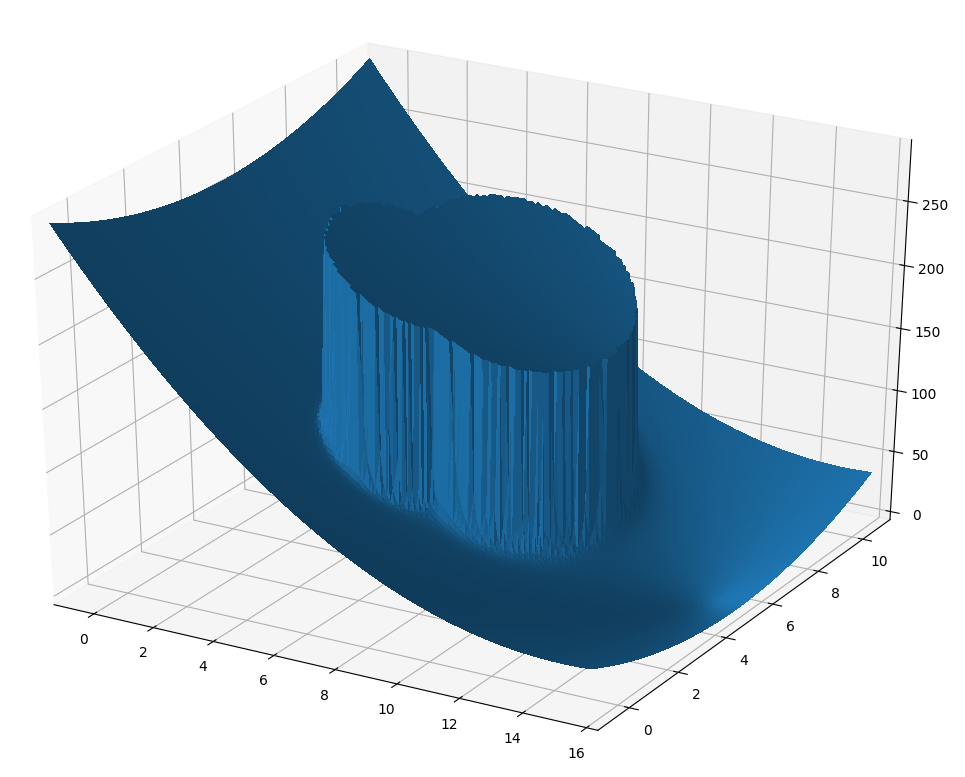
\includegraphics[scale=1]{field_obstacles}
    \caption{Potential Field with Obstacles}
    \label{fig:pot_field}
\end{figure}

There was a \textbf{lot} of testing because I incorrectly entered an obstacle 
formula into a partial derivative calculator. After finally getting it working I 
had to tweak $\gamma$ until it was able to make it through gradient decent. 
$\gamma$ is sometimes called $\alpha$ or \textit{step size}. Once I got it 
to descend to the goal I had to optimize it (of course). First I tried different 
static $\gamma$ values with varrying degrees of success. The real breakthrough 
came with Figure \ref{fig:expl}, where I applied the following:

$$\gamma = \ddfrac{1}{(x_0 - x_{goal})^2 + (y_0 - y_{goal})^2}$$

\begin{figure}[h]
    \centering
    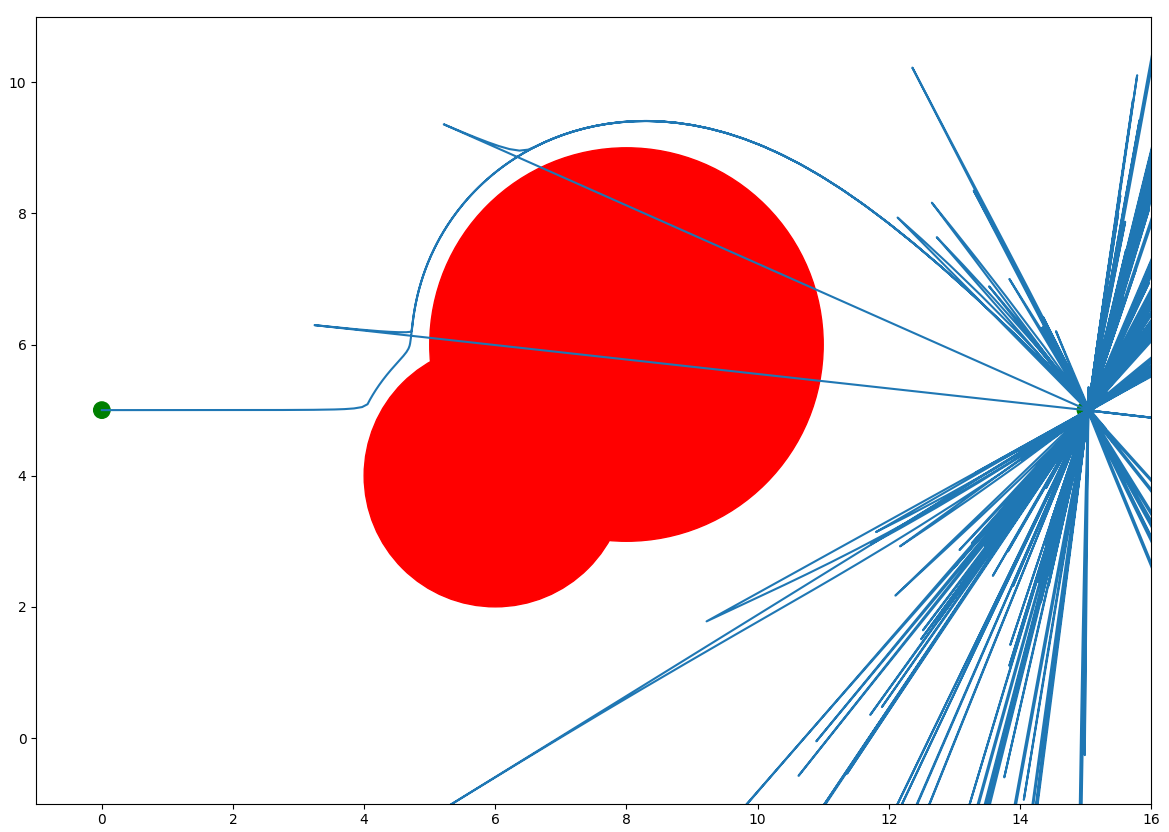
\includegraphics[scale=1]{explosion}
    \caption{Explosion}
    \label{fig:expl}
\end{figure}

I realized that as the distance to goal decreased it would generate exceedingly 
large $\gamma$ values. This was resolved with stepping the function:

$$
\[ \begin{cases} 
      \ddfrac{1}{(x_0 - x_{goal})^2 + (y_0 - y_{goal})^2} & D > \eta \\
      \gamma * 0.9 & 0.01 < D < \eta \\
      0 & D <= 0.01
   \end{cases}
\]
$$

Using this combination for $\gamma$ I was able to converge in a very reasonable 
174 steps. Figure \ref{fig:ppp} shows the start and end points in green, the 
path in blue, and the obstacles in red.

\begin{figure}[h]
    \centering
    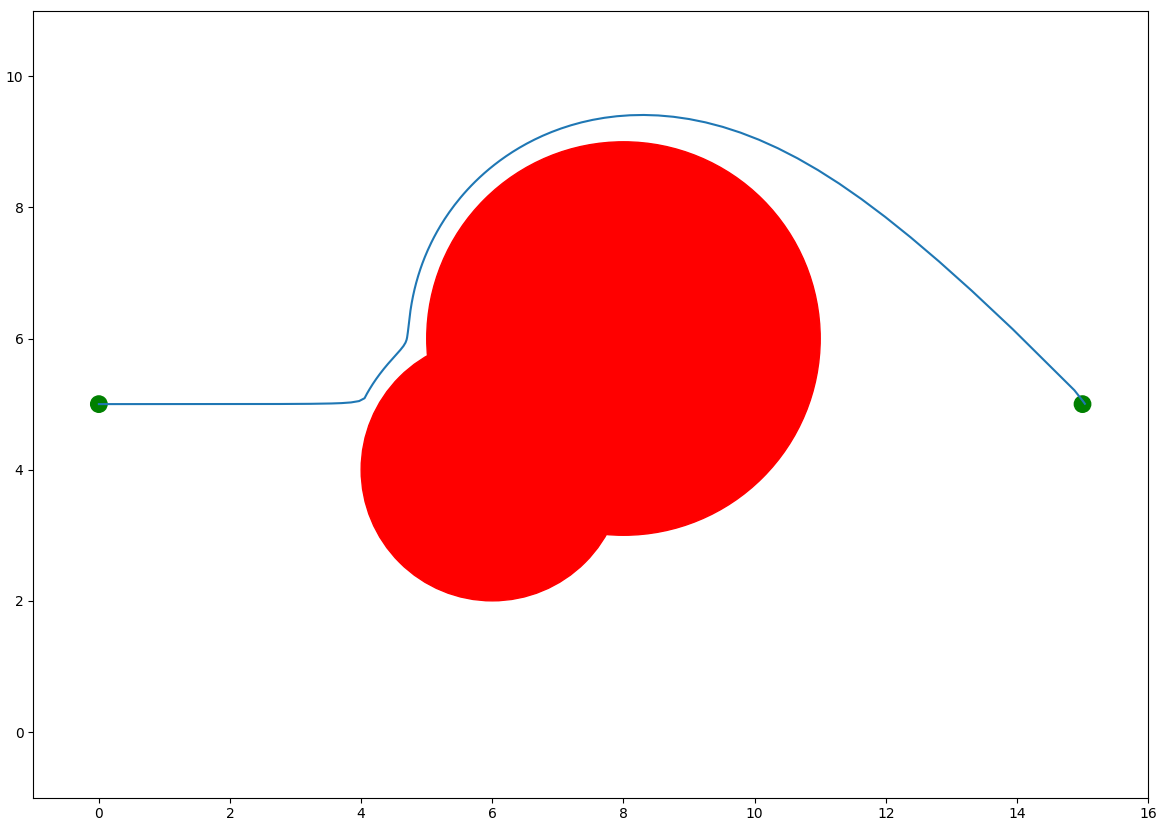
\includegraphics[scale=1]{best_path}
    \caption{Proper Path Planned}
    \label{fig:ppp}
\end{figure}



\end{document}
